%
%\documentclass[11pt,twoside,titlepage]{article}
\documentclass[11pt]{article}
\usepackage{a4,amssymb,rotating}
% \usepackage{epsfig,subfigure,fancyheadings}
\usepackage{epsfig,subfigure}
\usepackage{graphicx,color}
\usepackage{lineno}

\setlength{\oddsidemargin}{+0.3cm}
\setlength{\evensidemargin}{-0.3cm}
\setlength{\textwidth}{15.5cm}
\setlength{\textheight}{22.5cm}
\setlength{\topmargin}{-2.0cm}

\newif\ifcomment
\commenttrue % comment to remove comments

\newif\iflinenumber
\linenumbertrue % comment to remove line numbering

\newcommand{\comment}[1]{\ifcomment \color{blue}{\underline{Comment:} #1}\color{black}\fi}

\begin{document}
\sloppy
% \linenumbers

\title{{\bf FSA - Allergies and Social Media}}

\author{Newman Andrew\\ P\'erez~P\'erez Luis Alejandro\\ Pervane Ozge\\ Swar Toufik}

\date{Nov. 15th 2018}

% \begin{figure}
%   \centering
%     \includegraphics[width=0.7\textwidth]{figures/Guariguanchi_logo.png}
% \end{figure}

\maketitle

% \newpage

\begin{abstract}
The team is composed of Alejandro, Andrew, Ozge and Toufik.
\end{abstract}

\newpage

\tableofcontents

\newpage

\section{Introduction}
\label{sec:Intro}

Using social media data, FSA wants to be able to track endorcement of allergen based legislations in the UK.
There are two streams of analysis involved in this project :

\subsection{Stream 1}
\label{subsec:stream1}
Using social media data, we would like to determine whether some Local Authorities face more allergy-relate issues than others by tracking:

\begin{itemize}
  \item {\bf Allergy enquiries:} Do consumers experience negative or positive reactions from staff when enquiring about allergen information in restaurants/ food outlets?
  \item {\bf Food labelling:} Do consumers face issues with incorrect or incomplete food labelling?
  \item {\bf Reporting reactions:} Do consumers report allergic reactions to food or near-misses?
\end{itemize}

\subsection{Stream 2}
\label{subsec:stream2}
Based on a list of 14 common allergens provided in the EU legislation, we will focus on these 2 areas:

\begin{itemize}
  \item How much are each of the 14 allergens being talked about, and are they usually mentioned in isolation or in combination with others? What insight can we gain by analysis of posts relating to these 14 allergens?
  \item Are other allergens outside of this list of 14 being talked about? We will explore this by: (a) using a list of other likely allergenic foods provided by subject matter experts, and (b) for posts that do not contain any of the main 14, are there any common food themes. Are any of these mentioned more than any of the 14 allergens?
\end{itemize}


\section{Data Cleaning and Preprocessing}
\label{sec:preprocessing}

\subsection{Cleaning}
\label{subsec:cleaning}

First step of our code is too import the data provided by FSA in Excel Format and to load it in a DataFrame.
This will allow us to perform the data cleaning, which is composed of the following steps:

\begin{itemize}
  \item Remove of undesiered columns
  \item Ordering of data per dates
  \item Lowercasing of content
  \item Removal of undesired characters from including Emoticons, Hashtags, URLs, HTML tags and symbols and punctuation
  \item Removal of duplicates
  \item Removal of spaces around conten (Trimming)
\end{itemize}

For further future analysis, some information like Username and Hashtags are extracted in inserted in a new column.

Lots of content is composed of abbraviations. In order to be the more relevant possible in the future analysis, we convert those to there expander meaning for e.g. "asap" becomes "as soon as possible"

\subsection{Normalization}
\label{subsec:normalization}

The normalization  refers to the transformation of words into a more uniform form.

We perform stop words removals where words like "the" "an" and other articles are removed from the content. This allows compuation to be more efficiant, reducing content size.

We apply the stemming process, an algorithm that converts inflected forms of words into their base forms (stems). This allows us to discard variations of words (like singular, plural).

The words are treated like normalized elements that we call tokens.

We need to convert this set of tokens to a corpus in order to perform matricial analysis.

\subsection{Document Term Matrix}
\label{subsec:DTM}

After all our data is cleaned and preprocessed, our corpus is converted into a Data Term Matrix. A DTM is a matrix in which rows are documents, columns are terms, and cells indicate how often each term occurred in each document. In our case each line represents a tweet, forum entry or news.

This is the base element that we will use for Stream 1 and Stream 2 analyis.


\section{Data Analysis}
\label{sec:data_analysis}

\subsection{Supporting local authorities}
\label{subsec:supp_local_autho}

\subsubsection{Approach}

The idea is to use provided data in order to find out information about:
\begin{enumerate}
  \item Allergy enquiries
  \item Food labelling
  \item Reporting reactions
\end{enumerate}

Our approach was to use each of these elements and to find words related to the subject.

Let's take Food labelling as an example. The idea is to find cases where consumers face issues due to incorrect food labelling.

We divided it into the following list:

{\tt c("consumer", "issue", "labelling", "allergy")}

We used a Google library called Word2Vec an efficient implementation of the continuous bag-of-words and skip-gram architectures for computing vector representations of words.

For each of the words consumer, issue, labelling and allergen, we used word2vec to generate dictionaries of words with a strong semantic proximity.

If we talk the word allergy, applying word2vec functions to it provided us with a list of words related to the allergen subject.
With some data cleaning and manual rework, we obtain a dictionary with key and values.

Example for allergy : {\tt allergy,allergen,allergenic,allergens,allergic,allergies,allergy,}

This processed is applied to all the words that we will use to identify issues with food labelling.

We will generate a DFM composed of the list of all the entries (tweets, news, forum) by line, the column will be the key of our dictionary (in that case "allergy")
Because some of these may be repeted several times in a same document tweet or forum posts, the DFM is **normalized** containing 1 for  any occurence of the word >= 1. The matrix is composed of 0 and 1, corresponding to the occurrences of the context words.

\subsubsection{Labelling}

Using the previous generated matrix, we will apply the following logic to filter and label the tweets as per their corresponding context.

Staying in the example of food labelling, we apply the following logical expression :

{\tt \[(consurmer AND issue AND labelling) OR (incorrect AND allergy AND labelling) OR (consumer AND allergy AND labelling)\]}

When one of the above conditions is verified, we flag the corresponding document (tweet, or post forum) with the food\_labelling value to 1

The same process is applyied for the allergies inqueries and reactions reports.

\subsection{Identifying common allergens}
\label{subsec:allergens_mentions}

A similar approach is used to identify common allergens. The difference is that we already know the predefined list of keywords we are looking for.

In that case, we built dictionaries for the 14 allergens provided, and for the other list of allergens using the same principal as in first stream.

celery: {\tt celery,celeri}.

cereals containing gluten: {\tt wheat,rye,barley,barli,oat}


\section{Results}
\label{sec:results}

\subsection{Allergen Enquiries diplayed by Source and Sentiment}

\subsection{Food Labelling diplayed by Source and Sentiment}

\subsection{Allergen Enquiries, Food Labelling and Reactions Reporting combined by sentiment class}


kksll



\subsection{14 allergens}

In the representation below, we display the number of mentions of predefined list of 14 allergens, whether coming from Blog, News, Review, Forum or Twitter.

\begin{figure}
  \centering
  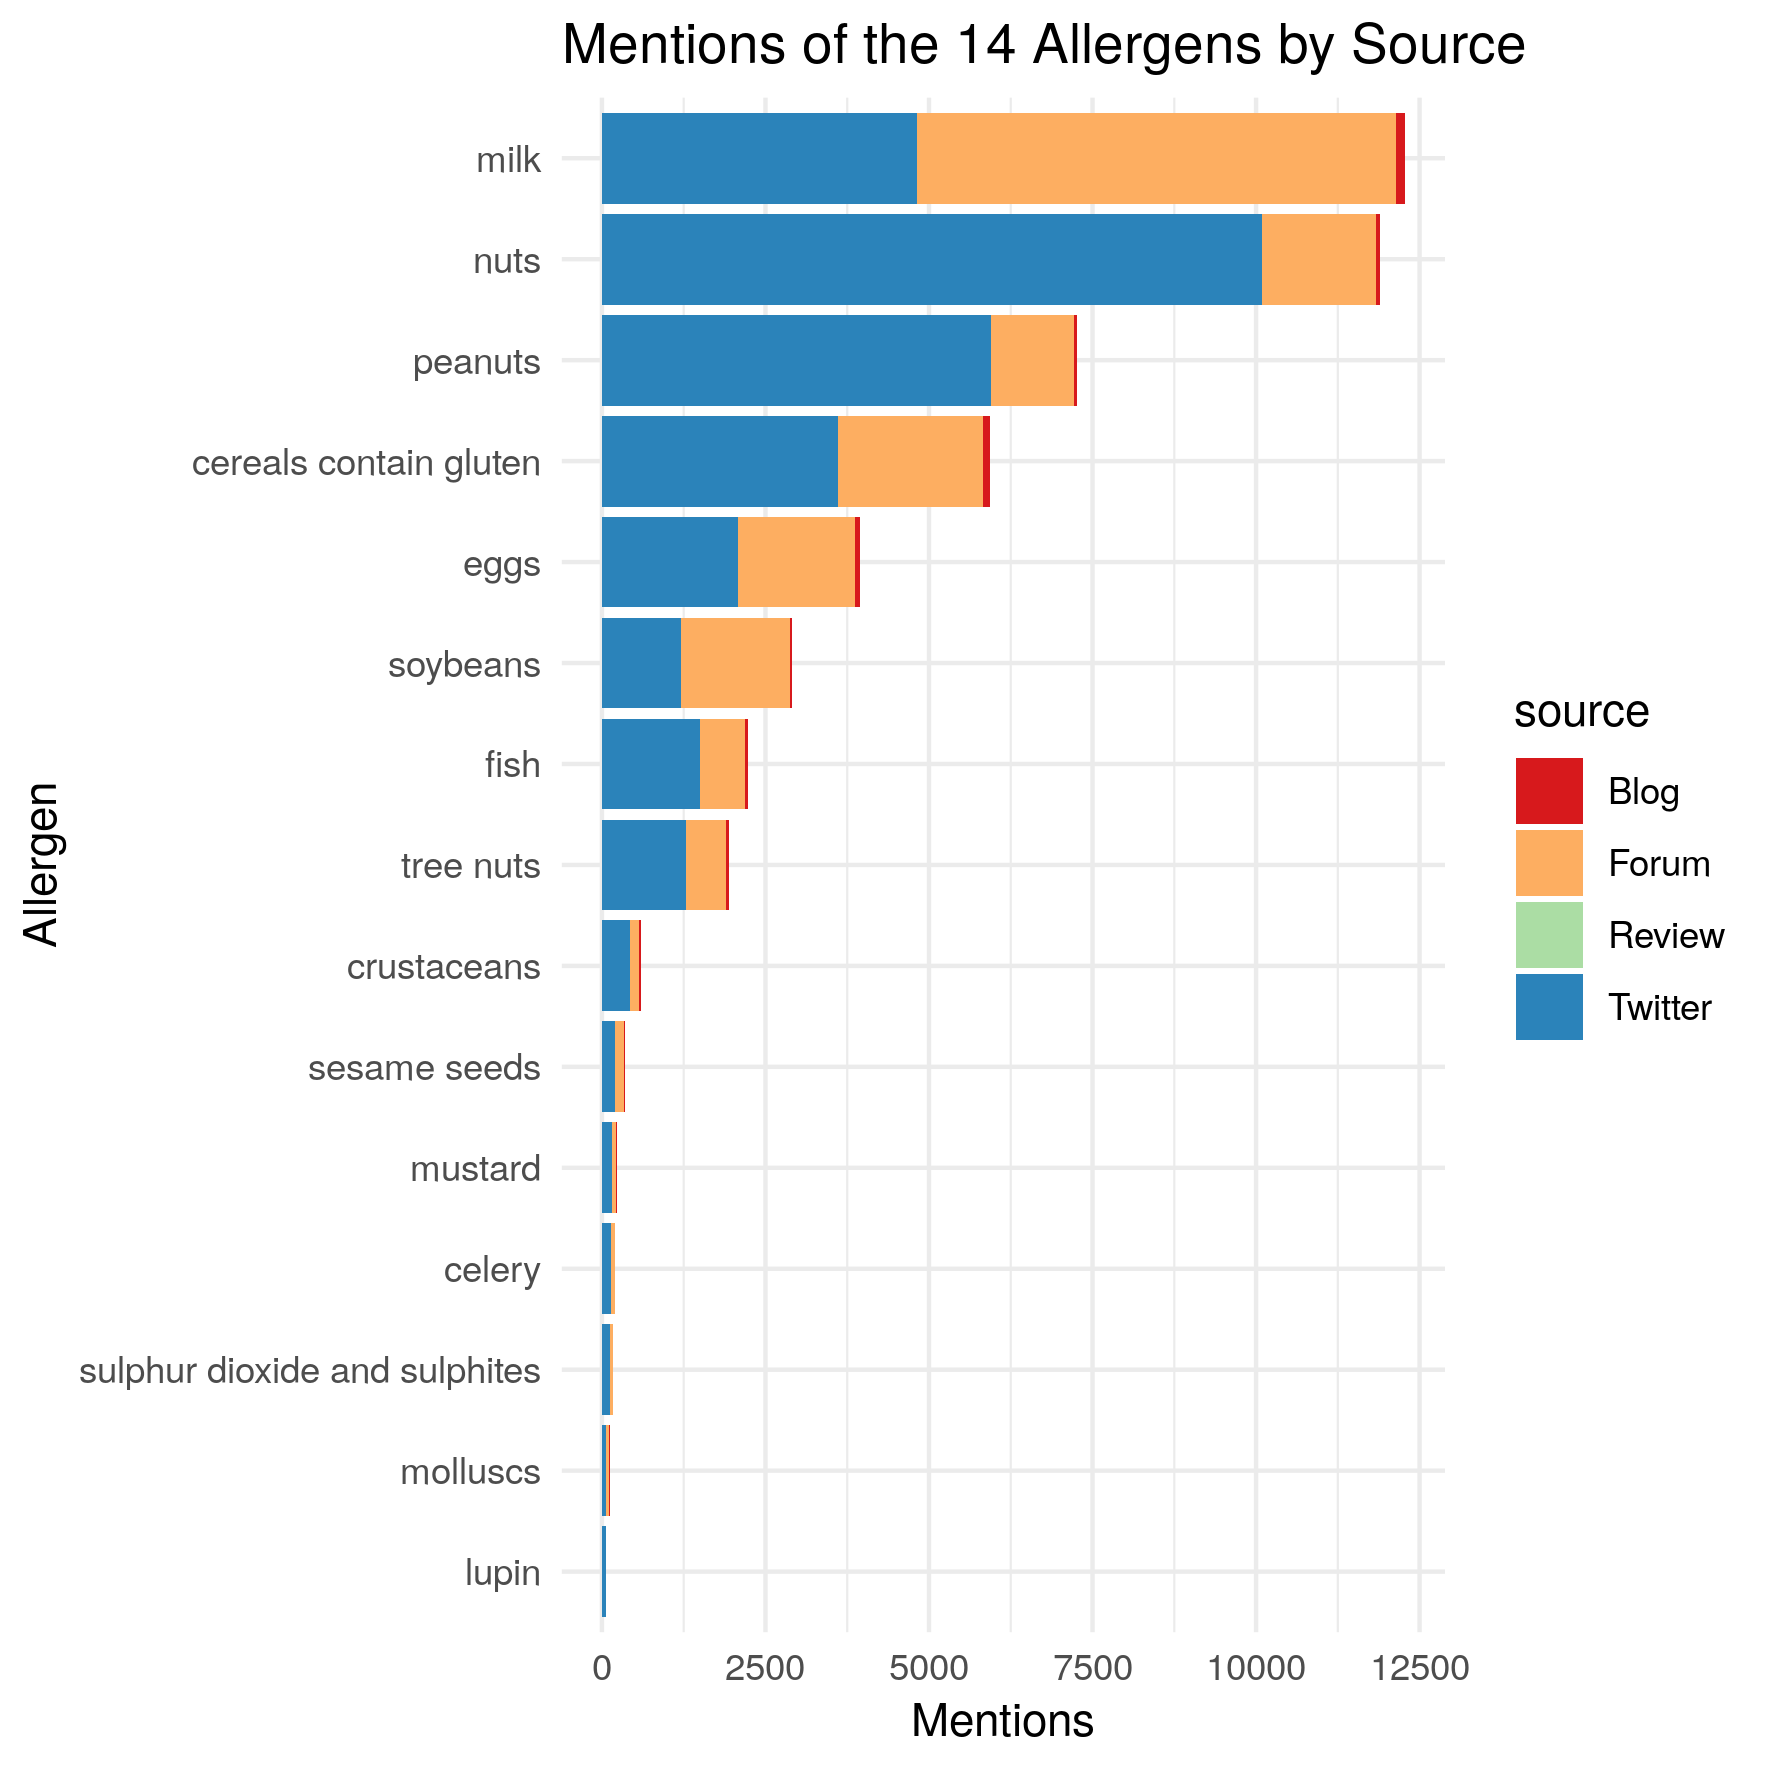
\includegraphics[width=0.6\textwidth]{figures/Dataset1/14_allergens_bysource.png}
  \caption{A nice plot ...}
\end{figure}

\subsection{Other Allergens}

\subsection{TOP 10 Allergens}

\subsection{14 Allergens Mentions over time (Twitter only)}

\subsection{Other Allergens Mentions over time (Twitter only)}


kmsjk



\subsection{Percentage of 14 allergens mentions for which we have a mild/severe reaction}

\subsection{Reactions to 14 Allergens Mentions over time from all sources}

\subsection{Reactions to the 14 Allergens over time, including all sources}

\subsection{Reactions to the 14 Allergens over time, including all sources and flagged under Food Labelling}

\subsection{Reactions to the 14 Allergens over time, including all sources and flagged under Allergy Enquiries}

\subsection{Reported Reactions to Other Allergens Over Time (All Sources)}



\section{Acknowledgements}
\label{sec:acknowledgements}

Bla bla bla


%%%%%%%%%%%%%%%%%%%%%%%%%%%%%%%%
\begin{thebibliography}{00}
%%%%%%%%%%%%%%%%%%%%%%%%%%%%%%%%

\bibitem{bib:ILDcoll} fff

\end{thebibliography}


\end{document}
